\documentclass{ctexbeamer}

% 使用 <thubeamer> 主题
% 模板选项如下
% (a.1) smoothbars: 页面顶端单行显示目录，默认选项
\usetheme[sectiontoc]{thubeamer}

\usepackage{media9}
\usepackage{listings}
\usepackage{multirow}
\usepackage{colortbl}
\usepackage{booktabs}
\lstnewenvironment{textcode}{
  \lstset{
    basicstyle=\footnotesize\ttfamily,
    breaklines=true,
    frame=single,
    numbersep=2pt,
    xleftmargin=0.5em,
    framesep=1mm
  }
}{}


% (a.2) sidebar: 页面左侧分栏显示目录
% \usetheme[sidebar]{thubeamer}

% (b) sectiontoc: 在每节（section）前显示目录，并高亮显示当前节，默认不显示

% (c) subsectiontoc: 在每小节（subsection）前显示目录，并高亮显示当前节和当前小节，默认不显示

% (d) en: 仅使用英文来制作 beamer，应用此选项后，汉字将全部无法编译

% 图片存放路径

\graphicspath{{figures/}}

\include{macros}

% 封面信息，方括号内容是显示在左侧边栏的内容（当选择 sidebar 主题时有效）
\title[篮球高光检测]{篮球高光检测项目\\[2mm] 汇报}
\author[唐梓楠]{牛衍昌\\鲁继元\\唐梓楠\\[5mm] 导师：黄必清教授}
\institute[清华大学]{\small 清华大学}
\date{\small \vskip -10pt \today}

% 开始写文章
\begin{document}

% 标题页
\begin{frame}
  \maketitle
\end{frame}

% 目录页
\section*{目录}
\frame{
  \frametitle{\secname}
  \tableofcontents[hideallsubsections]
}

\section{Paper Sharing: Multi-View 3D Point Tracking}

\begin{frame}{MVTracker}
  \begin{block}{ICCV 2025 (Oral)}
    \textbf{Multi-View 3D Point Tracking}~\cite{Rajic_2025_ICCV}
  \end{block}
  \vspace{0.3cm}
  \begin{columns}[T]
    \begin{column}{0.5\textwidth}
      \textbf{主要贡献}
      \begin{itemize}
        \item 首个\alert{数据驱动}的多视角3D点追踪器
        \item 无需逐序列优化，支持前馈推理
        \item 仅需4个相机视角即可达到高精度
      \end{itemize}
    \end{column}
    \begin{column}{0.5\textwidth}
      \textbf{项目资源}
      \begin{itemize}
        \item 代码、模型、数据集开源
        \item \url{ethz-vlg.github.io/mvtracker}
      \end{itemize}
      \vspace{0.2cm}
      \textbf{性能指标}
      \begin{itemize}
        \item Panoptic Studio: MTE 3.1cm
        \item DexYCB: MTE 2.0cm
        \item 推理速度: 7.2 FPS
      \end{itemize}
    \end{column}
  \end{columns}
\end{frame}

\begin{frame}{研究动机}
  \begin{columns}[T]
    \begin{column}{0.5\textwidth}
      \textbf{现有方法的局限性}
      \begin{enumerate}
        \item \textbf{单目追踪器}: 
        \begin{itemize}
          \item 深度歧义严重
          \item 遮挡处理困难
          \item 3D一致性差
        \end{itemize}
        \item \textbf{多相机优化方法}:
        \begin{itemize}
          \item 需要20+个相机
          \item 逐序列优化耗时
          \item 不适合实时应用
        \end{itemize}
      \end{enumerate}
    \end{column}
    \begin{column}{0.5\textwidth}
      \textbf{MVTracker的优势}
      \begin{itemize}
        \item \alert{前馈模型}：直接预测3D对应关系
        \item \alert{少量相机}：仅需4个视角
        \item \alert{在线追踪}：适合实际应用
        \item \alert{鲁棒性强}：处理遮挡和深度噪声
      \end{itemize}
      \vspace{0.3cm}
      \textbf{应用场景}
      \begin{itemize}
        \item 动态场景重建
        \item 机器人技术
        \item 增强现实
      \end{itemize}
    \end{column}
  \end{columns}
\end{frame}

\begin{frame}{Teaser: 多视角3D点追踪效果}
  \begin{figure}
    \centering
    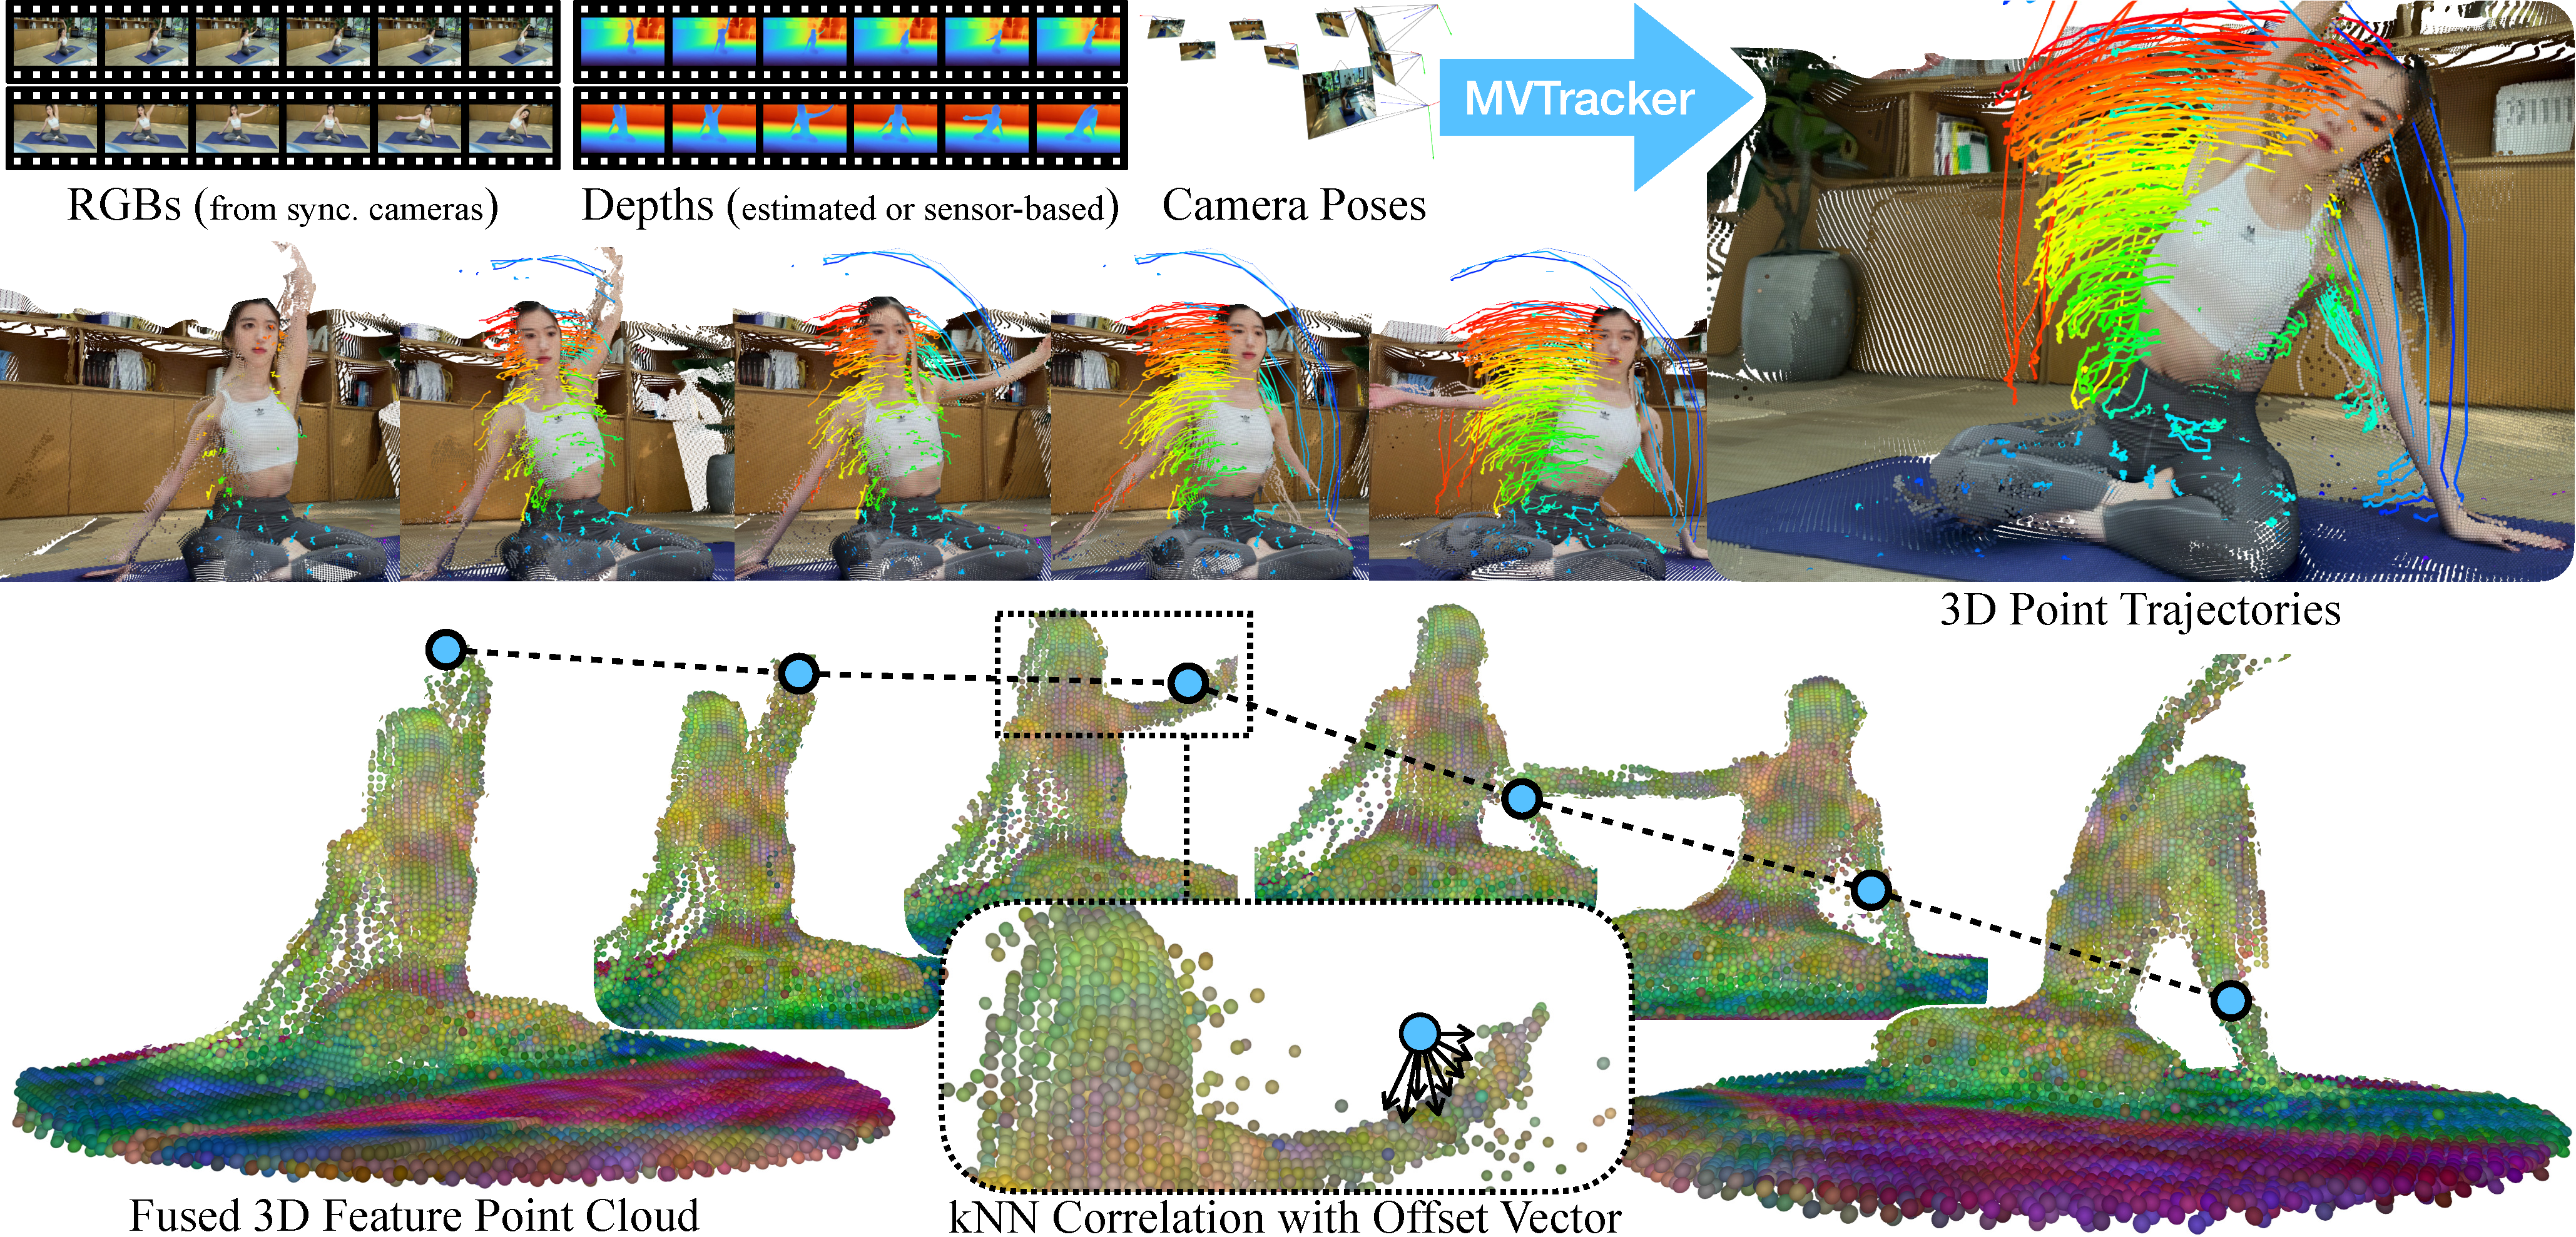
\includegraphics[width=0.95\textwidth]{figures/teaser__july_25.optimized-prepress.pdf}
    \caption{MVTracker在SelfCap数据集上的追踪结果，使用DUSt3R估计深度}
  \end{figure}
\end{frame}

\begin{frame}{方法框架}
  \begin{figure}
    \centering
    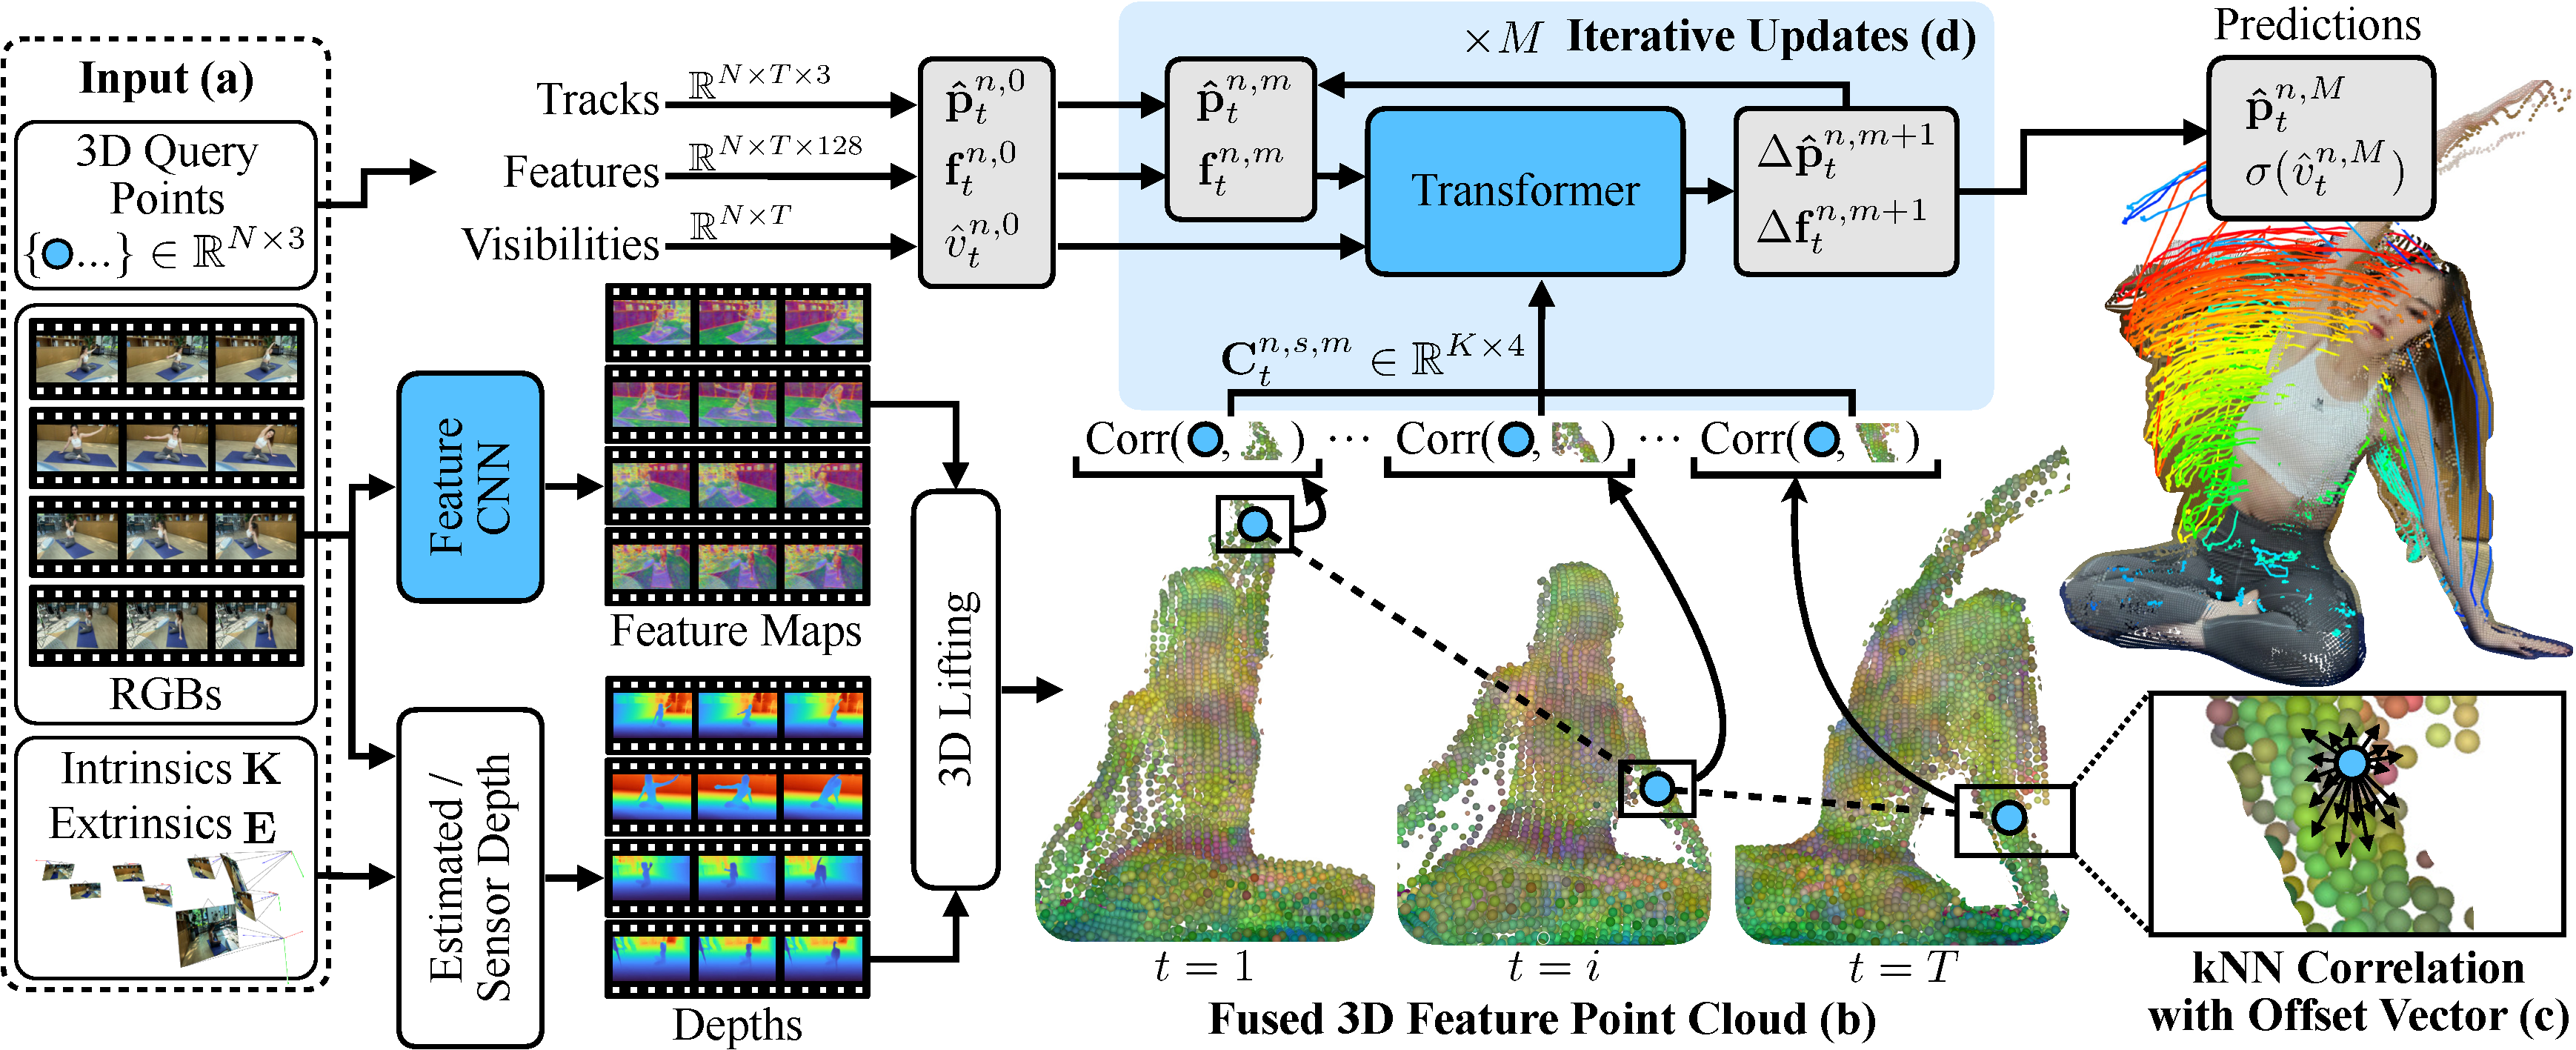
\includegraphics[width=\textwidth]{figures/pipeline_july_v3.optimized-prepress.pdf}
    \caption{MVTracker整体流程}
  \end{figure}
\end{frame}

\begin{frame}{点云特征融合}
  \textbf{核心思想}: 将多视角RGB-D数据融合为统一的3D特征点云
  \vspace{0.3cm}
  
  \begin{columns}[T]
    \begin{column}{0.5\textwidth}
      \textbf{(a) 特征提取}
      \begin{itemize}
        \item CNN编码器提取每视角特征图
        \item 多尺度特征 (4个尺度)
        \item 分辨率：$\frac{H}{4} \times \frac{W}{4}$
      \end{itemize}
      \vspace{0.2cm}
      \textbf{(b) 点云构建}
      \begin{itemize}
        \item 深度估计或传感器深度
        \item 像素反投影到3D空间
        \item 关联特征向量
      \end{itemize}
    \end{column}
    \begin{column}{0.5\textwidth}
      \textbf{融合公式}
      \begin{equation*}
        \mathcal{X}_t^s = \{(\mathbf{x}, \Phi_t^{v,s}[u_y,u_x])\}
      \end{equation*}
      
      \textbf{优势 vs Triplane}
      \begin{itemize}
        \item \alert{避免投影碰撞}：不同3D点映射到同一2D平面位置
        \item \alert{自适应场景}：无需预定义边界区域
        \item \alert{保留完整特征}：无信息损失
      \end{itemize}
    \end{column}
  \end{columns}
\end{frame}

\begin{frame}{kNN关联机制}
  \textbf{核心创新}: 基于k近邻的多尺度空间关联
  \vspace{0.2cm}
  
  \begin{columns}[T]
    \begin{column}{0.55\textwidth}
      \textbf{关联计算}
      \begin{equation*}
        \mathbf{C}_t^{n,s} = \{\langle \mathbf{f}_t^n, \mathbf{\phi}_k \rangle | (\mathbf{x}_k, \mathbf{\phi}_k) \in \mathcal{N}_K(\hat{\mathbf{p}}_t^n, \mathcal{X}_t^s)\}
      \end{equation*}
      
      \textbf{偏移编码}
      \begin{itemize}
        \item 每个近邻关联: 相似度 + 3D偏移向量
        \item 偏移向量: $\mathbf{x}_k - \hat{\mathbf{p}}_t^n$
        \item 编码方向和距离信息
      \end{itemize}
    \end{column}
    \begin{column}{0.45\textwidth}
      \textbf{多尺度覆盖范围}
      \begin{table}
        \footnotesize
        \begin{tabular}{cc}
          \hline
          尺度 & 平均距离 (cm) \\
          \hline
          Scale 1 & $12.5 \pm 8.2$ \\
          Scale 2 & $22.4 \pm 12.2$ \\
          Scale 3 & $42.7 \pm 21.7$ \\
          Scale 4 & $85.8 \pm 44.0$ \\
          \hline
        \end{tabular}
      \end{table}
      最大尺度可覆盖约92 km/h的运动
    \end{column}
  \end{columns}
  
  \vspace{0.3cm}
  \textbf{vs 2D/Triplane关联}
  \begin{itemize}
    \item 2D关联可能匹配到不相关的背景像素
    \item Triplane关联存在固有的信息损失
    \item \alert{kNN直接在3D空间搜索几何相关的邻域}
  \end{itemize}
\end{frame}

\begin{frame}{方法详解 (3): Transformer迭代更新}
  \begin{columns}[T]
    \begin{column}{0.5\textwidth}
      \textbf{Token构建}
      \begin{equation*}
        G_t^n = (\eta(\hat{\mathbf{p}}_t^n - \hat{\mathbf{p}}_{t_n^q}^n), \mathbf{f}_t^n, \mathbf{C}_t^{n,s}, \hat{v}_t^n)
      \end{equation*}
      
      \textbf{更新机制}
      \begin{itemize}
        \item 时序自注意力
        \item 虚拟轨迹交叉注意力
        \item 迭代残差更新
      \end{itemize}
      
      \textbf{迭代更新公式}
      \begin{align*}
        \hat{\mathbf{p}}_t^{n,m+1} &= \hat{\mathbf{p}}_t^{n,m} + \Delta\hat{\mathbf{p}}_t^{n,m+1} \\
        \mathbf{f}_t^{n,m+1} &= \mathbf{f}_t^{n,m} + \Delta\mathbf{f}_t^{n,m+1}
      \end{align*}
    \end{column}
    \begin{column}{0.5\textwidth}
      \textbf{滑动窗口推理}
      \begin{itemize}
        \item 窗口大小: $T=12$ 帧
        \item 重叠: $T/2$ 帧
        \item 长视频分割处理
      \end{itemize}
      
      \vspace{0.3cm}
      \textbf{可见性预测}
      \begin{equation*}
        \hat{v}_t^n = \sigma(W \mathbf{f}_t^{n,M})
      \end{equation*}
      
      \vspace{0.2cm}
      \textbf{训练设置}
      \begin{itemize}
        \item 数据集: MV-Kub (5K序列)
        \item 200K训练步
        \item 8×GH200 GPU, 8天
      \end{itemize}
    \end{column}
  \end{columns}
\end{frame}

\begin{frame}{实验结果: 主要对比}
  \begin{table}
    \centering
    \footnotesize
    \setlength{\tabcolsep}{3pt}
    \caption{多视角3D点追踪性能对比 (MTE单位: cm)}
    \begin{tabular}{l|cccc|cccc}
      \hline
      \multirow{2}{*}{方法} & \multicolumn{4}{c|}{Panoptic Studio} & \multicolumn{4}{c}{DexYCB} \\
      & AJ$\uparrow$ & $\delta_{avg}\uparrow$ & OA$\uparrow$ & MTE$\downarrow$ & AJ$\uparrow$ & $\delta_{avg}\uparrow$ & OA$\uparrow$ & MTE$\downarrow$ \\
      \hline
      Dynamic 3DGS & 66.5 & 92.4 & 74.1 & 3.9 & 45.7 & 57.1 & 81.3 & 11.3 \\
      Shape of Motion & 72.6 & 89.2 & 82.1 & 4.8 & 36.2 & 53.6 & 63.3 & 8.0 \\
      CoTracker3 & 74.5 & 84.5 & 86.4 & 8.6 & 29.4 & 40.3 & 78.6 & 22.0 \\
      SpaTracker & 61.5 & 82.3 & 75.5 & 7.3 & 58.3 & 72.0 & 80.2 & 5.9 \\
      TAPIP3D & 84.3 & 93.8 & 91.4 & 3.1 & 38.8 & 50.0 & 90.1 & 8.2 \\
      Triplane Baseline & 65.1 & 81.8 & 82.8 & 7.2 & 57.5 & 71.0 & 81.3 & 4.3 \\
      \hline
      \rowcolor{cyan!20} \textbf{MVTracker} & \textbf{86.0} & \textbf{94.7} & \textbf{92.3} & \textbf{3.1} & \textbf{71.6} & \textbf{80.6} & \textbf{91.3} & \textbf{2.0} \\
      \hline
    \end{tabular}
  \end{table}
  
  \vspace{0.2cm}
  \textbf{关键发现}
  \begin{itemize}
    \item MVTracker在所有数据集上均达到\alert{最高精度}
    \item 相比单视角方法 (CoTracker3, SpaTracker) 提升显著
    \item 相比优化方法 (Dynamic 3DGS, SoM) 更快且更准确
  \end{itemize}
\end{frame}

\begin{frame}{定性结果对比}
  \begin{figure}
    \centering
    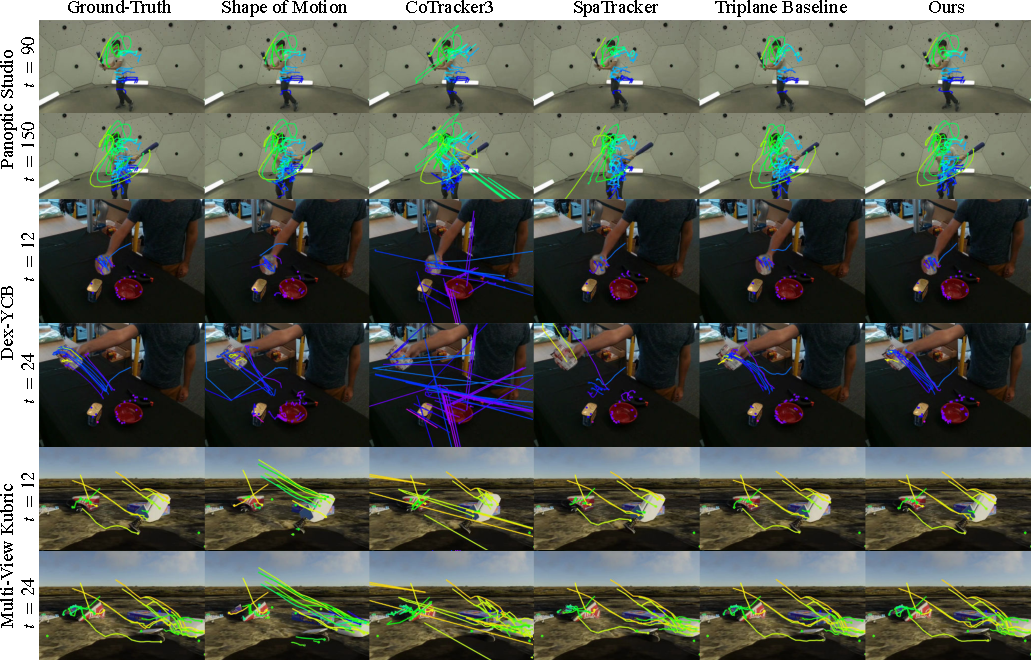
\includegraphics[width=0.95\textwidth]{figures/qualitative_comparison.optimized-printer.pdf}
    \caption{不同方法的追踪轨迹可视化对比}
  \end{figure}
\end{frame}

\begin{frame}{消融实验: 视角数量的影响}
  \begin{columns}[T]
    \begin{column}{0.55\textwidth}
      \begin{figure}
        \centering
        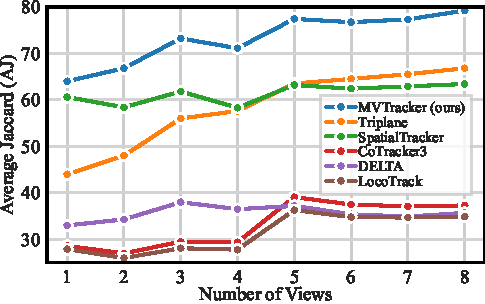
\includegraphics[width=\textwidth]{figures/plot_number_of_views.pdf}
        \caption{DexYCB上不同视角数的AJ性能}
      \end{figure}
    \end{column}
    \begin{column}{0.45\textwidth}
      \textbf{观察结果}
      \begin{itemize}
        \item MVTracker: 视角越多性能越好
        \item 1视角: AJ=64.0
        \item 4视角: AJ=71.1
        \item 8视角: AJ=79.2
      \end{itemize}
      
      \vspace{0.3cm}
      \textbf{对比分析}
      \begin{itemize}
        \item SpaTracker/Triplane: 性能较早饱和
        \item 单视角方法: 增加视角提升有限
        \item \alert{MVTracker扩展性最佳}
      \end{itemize}
    \end{column}
  \end{columns}
\end{frame}

\begin{frame}{消融实验: kNN关联组件}
  \begin{table}
    \centering
    \caption{关联组件对性能的影响 (MV-Kubric)}
    \begin{tabular}{l|cccc}
      \hline
      配置 & AJ$\uparrow$ & $\delta_{avg}\uparrow$ & OA$\uparrow$ & MTE$\downarrow$ \\
      \hline
      无偏移向量 & 72.9 & 80.5 & 93.9 & 2.7 \\
      偏移 + 绝对位置 & 74.7 & 82.7 & 93.5 & 2.3 \\
      \rowcolor{cyan!20} \textbf{仅偏移向量} & \textbf{77.3} & \textbf{85.0} & \textbf{94.4} & \textbf{1.9} \\
      \hline
    \end{tabular}
  \end{table}
  
  \vspace{0.3cm}
  \textbf{关键发现}
  \begin{itemize}
    \item 2D关联中方向隐式编码在像素网格中
    \item 3D kNN从各方向检索邻居，\alert{显式偏移信息至关重要}
    \item 仅使用相对偏移效果最佳，避免绝对位置干扰
  \end{itemize}
\end{frame}

\begin{frame}{深度估计的影响}
  \begin{columns}[T]
    \begin{column}{0.55\textwidth}
      \begin{figure}
        \centering
        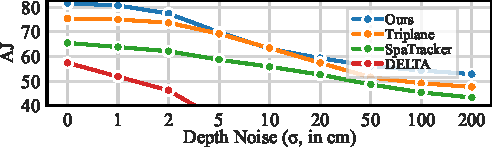
\includegraphics[width=\textwidth]{figures/plot_robustness_to_depth_noise.pdf}
        \caption{对深度噪声的鲁棒性 (MV-Kubric)}
      \end{figure}
    \end{column}
    \begin{column}{0.45\textwidth}
      \textbf{深度来源对比 (AJ)}
      \begin{table}
        \footnotesize
        \begin{tabular}{l|cc}
          \hline
          方法 & Sensor & DUSt3R \\
          \hline
          SpaTracker & 60.9 & 58.3 \\
          Triplane & 68.0 & 57.5 \\
          \textbf{MVTracker} & \textbf{82.7} & \textbf{71.6} \\
          \hline
        \end{tabular}
      \end{table}
      
      \vspace{0.2cm}
      \textbf{鲁棒性}
      \begin{itemize}
        \item 噪声$\sigma \leq 2$cm时性能稳定
        \item 支持多种深度来源
        \item 训练增强提升泛化能力
      \end{itemize}
    \end{column}
  \end{columns}
\end{frame}

\begin{frame}{推理速度对比}
  \begin{table}
    \centering
    \caption{运行时性能对比}
    \begin{tabular}{l|c|l}
      \hline
      方法 & FPS & 备注 \\
      \hline
      Dynamic 3DGS & - & 优化方法 (\~{}50分钟/序列) \\
      Shape of Motion & - & 优化方法 (\~{}30分钟/序列) \\
      SpaTracker & 1.4 & 单视角 \\
      DELTA & 1.5 & 单视角 \\
      CoTracker2 & 5.7 & 2D追踪器 \\
      Triplane Baseline & 5.8 & 多视角 \\
      \rowcolor{cyan!20} \textbf{MVTracker} & \textbf{7.2} & \textbf{多视角} \\
      CoTracker3 & 18.4 & 2D追踪器 \\
      \hline
    \end{tabular}
  \end{table}
  
  \vspace{0.2cm}
  \textbf{总结}: MVTracker实现了\alert{精度与速度的最佳平衡}，适合实时应用
\end{frame}

\begin{frame}{局限性与未来方向}
  \begin{columns}[T]
    \begin{column}{0.5\textwidth}
      \textbf{当前局限性}
      \begin{enumerate}
        \item \textbf{深度依赖}
        \begin{itemize}
          \item 依赖深度估计质量
          \item 稀疏视角下估计可能不可靠
        \end{itemize}
        \item \textbf{场景范围}
        \begin{itemize}
          \item 聚焦于有界区域
          \item 室外无界场景挑战大
        \end{itemize}
        \item \textbf{场景归一化}
        \begin{itemize}
          \item 需要手动或启发式变换
          \item 需更通用的方法
        \end{itemize}
      \end{enumerate}
    \end{column}
    \begin{column}{0.5\textwidth}
      \textbf{未来方向}
      \begin{itemize}
        \item 联合深度估计与追踪
        \item 4D重建基础模型
        \item 自监督学习减少合成-真实域差距
        \item 支持任意新场景
      \end{itemize}
      
      \vspace{0.3cm}
      \textbf{应用前景}
      \begin{itemize}
        \item 机器人学
        \item 优化重建方法的多视角先验
        \item 端到端4D重建模型
      \end{itemize}
    \end{column}
  \end{columns}
\end{frame}

\section{复现结果（进行中）}

\begin{frame}{复现进展概述}
  \begin{block}{当前状态}
    MVTracker 复现工作进行中，已完成部分环节
  \end{block}
  
  \vspace{0.3cm}
  \begin{columns}[T]
    \begin{column}{0.5\textwidth}
      \textbf{已完成}
      \begin{itemize}
        \item 环境配置与依赖安装
        \item MoGe 深度估计模块
        \item Demo 脚本运行
        \item 官方 Demo 数据验证
      \end{itemize}
    \end{column}
    \begin{column}{0.5\textwidth}
      \textbf{待解决}
      \begin{itemize}
        \item 多视角点云对齐问题
        \item 相机参数配置调整
        \item Query points 位置校正
        \item 自有数据集适配
      \end{itemize}
    \end{column}
  \end{columns}
  
  \vspace{0.3cm}
  \textbf{与项目的衔接点}：MVTracker 的 query\_points 追踪可与 YOLO 检测框结合，实现篮球等目标的 3D 轨迹追踪
\end{frame}

\begin{frame}{深度估计: MoGe}
  \begin{columns}[T]
    \begin{column}{0.55\textwidth}
      \begin{figure}
        \centering
        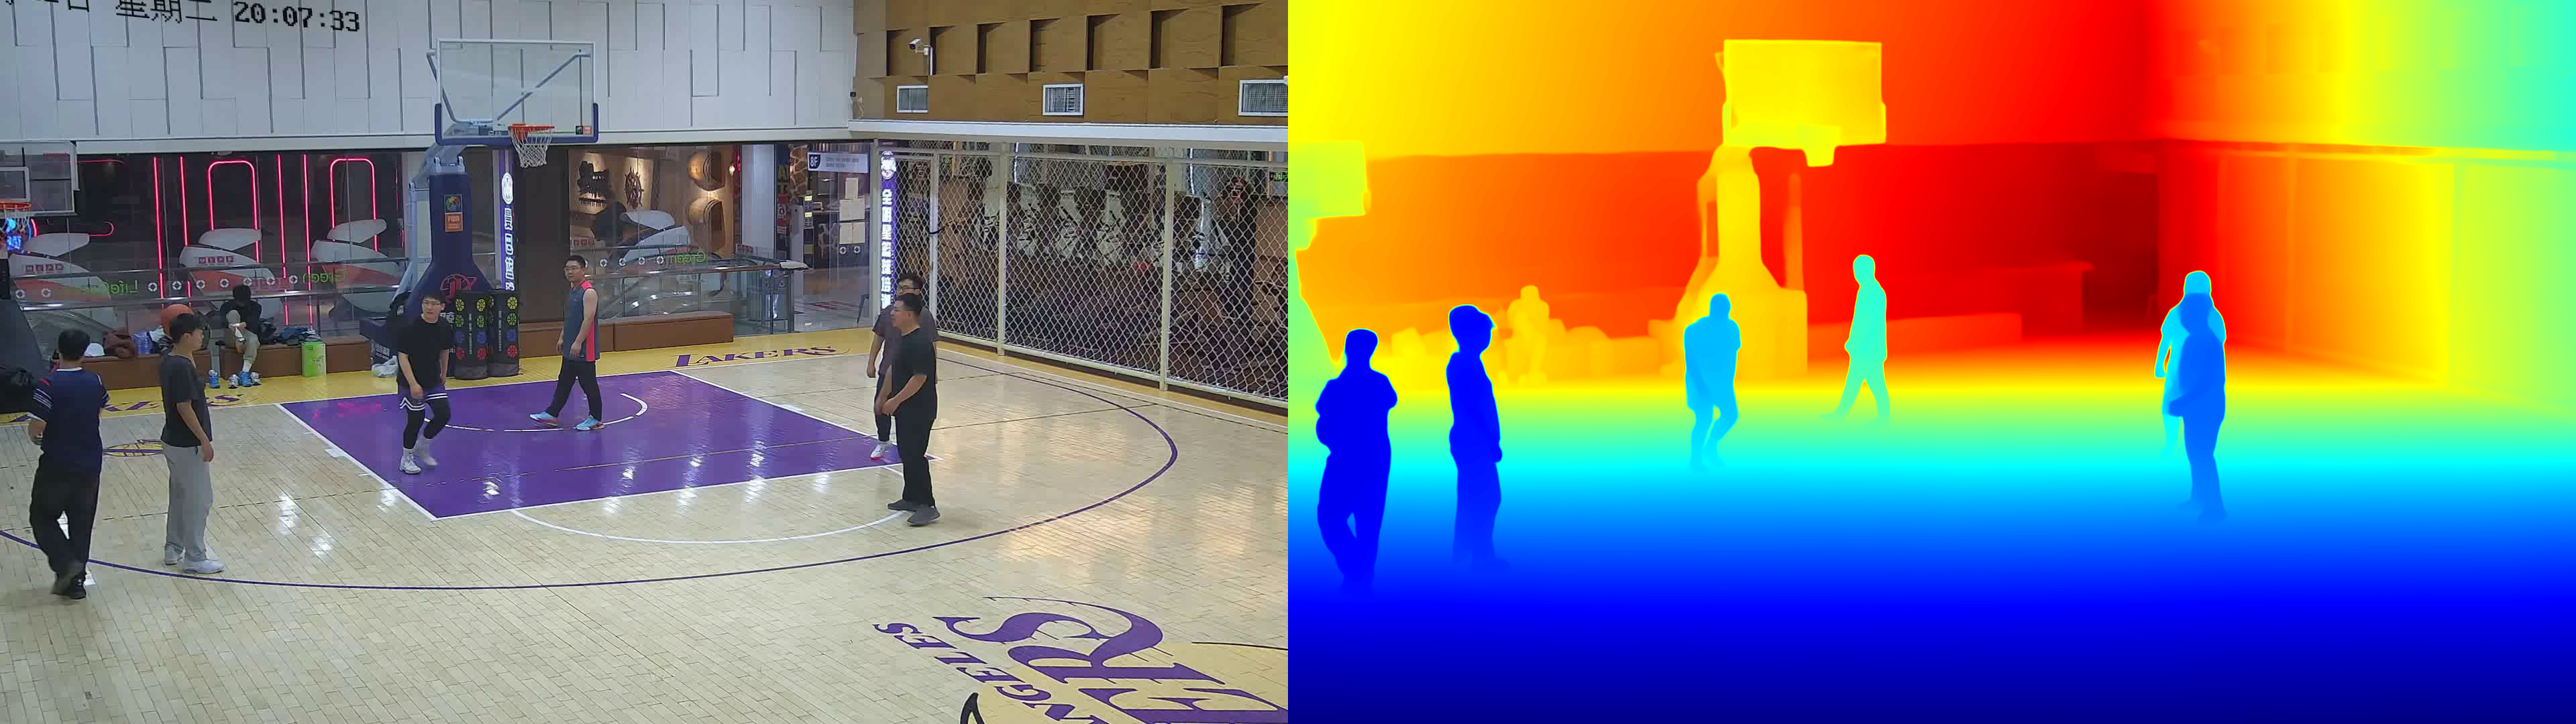
\includegraphics[width=\textwidth]{figures/depth_view0_frame000.png}
        \caption{MoGe 估计的深度图}
      \end{figure}
    \end{column}
    \begin{column}{0.45\textwidth}
      \textbf{深度估计方案}
      \begin{itemize}
        \item 使用 MoGe 进行单目深度估计
        \item 为每个视角生成深度图
        \item 深度信息用于点云构建
      \end{itemize}
      
      \vspace{0.3cm}
      \textbf{备选方案}
      \begin{itemize}
        \item DUSt3R: 0.17 FPS
        \item VGGT: 3.1 FPS (推荐)
        \item 传感器深度 (如有)
      \end{itemize}
    \end{column}
  \end{columns}
\end{frame}

\begin{frame}{官方 Demo 效果}
  \begin{columns}[T]
    \begin{column}{0.55\textwidth}
      \begin{figure}
        \centering
        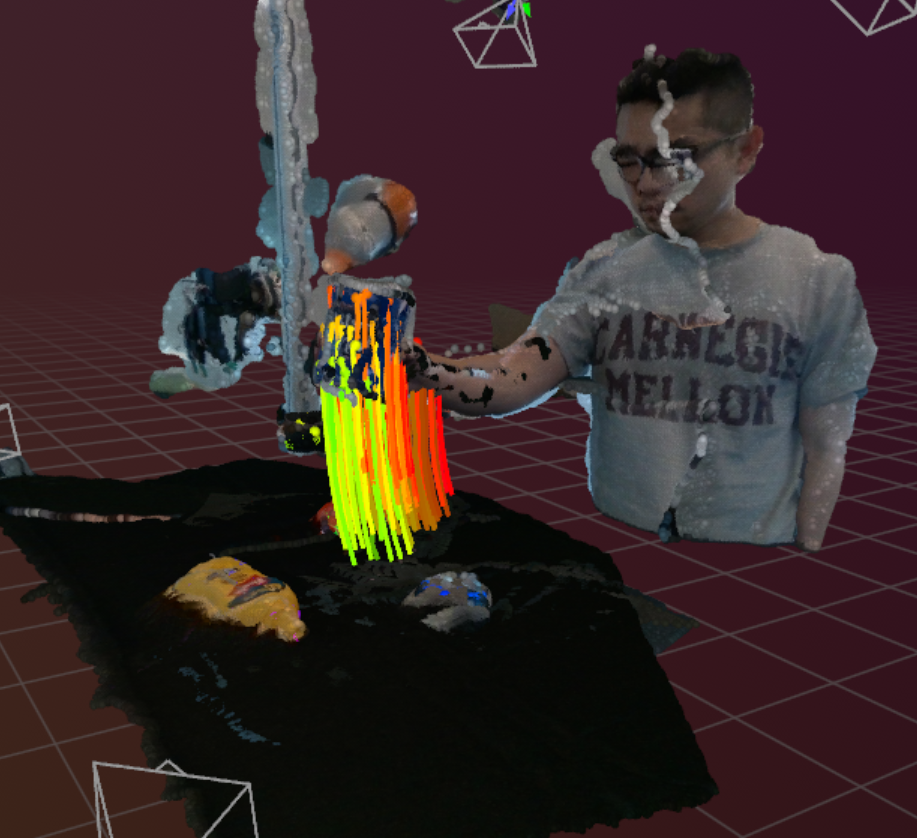
\includegraphics[width=\textwidth]{figures/demoscene.png}
        \caption{四相机 Demo 场景 (panoptic\_\_basketball)}
      \end{figure}
    \end{column}
    \begin{column}{0.45\textwidth}
      \textbf{Demo 配置}
      \begin{itemize}
        \item 数据集: Panoptic Studio
        \item 场景: basketball
        \item 相机数量: 4个视角
        \item 可视化: Rerun (.rrd)
      \end{itemize}
      
      \vspace{0.3cm}
      \textbf{效果说明}
      \begin{itemize}
        \item 多视角融合正确
        \item 点云场景完整
        \item 追踪轨迹清晰
      \end{itemize}
    \end{column}
  \end{columns}
\end{frame}

\begin{frame}{当前复现结果}
  \begin{columns}[T]
    \begin{column}{0.5\textwidth}
      \begin{figure}
        \centering
        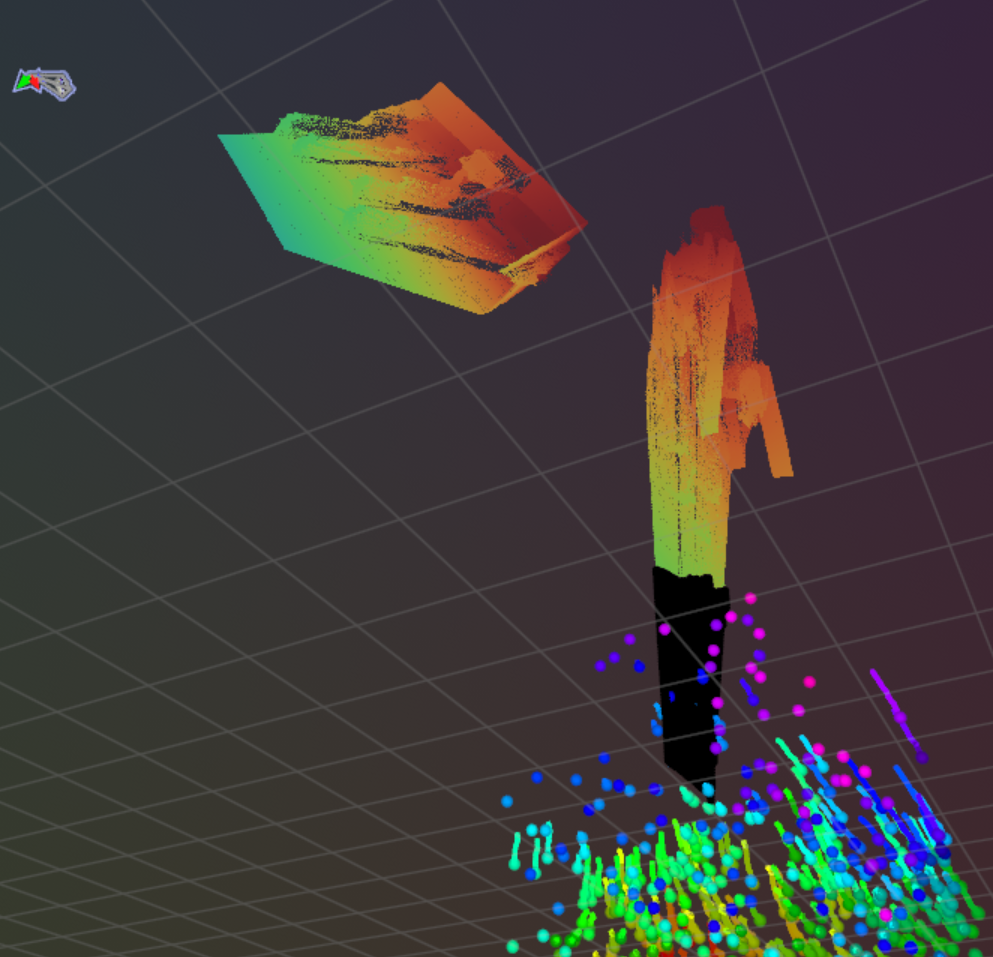
\includegraphics[width=\textwidth]{figures/uncompleted.png}
        \caption{当前输出 (整体视图)}
      \end{figure}
    \end{column}
    \begin{column}{0.5\textwidth}
      \begin{figure}
        \centering
        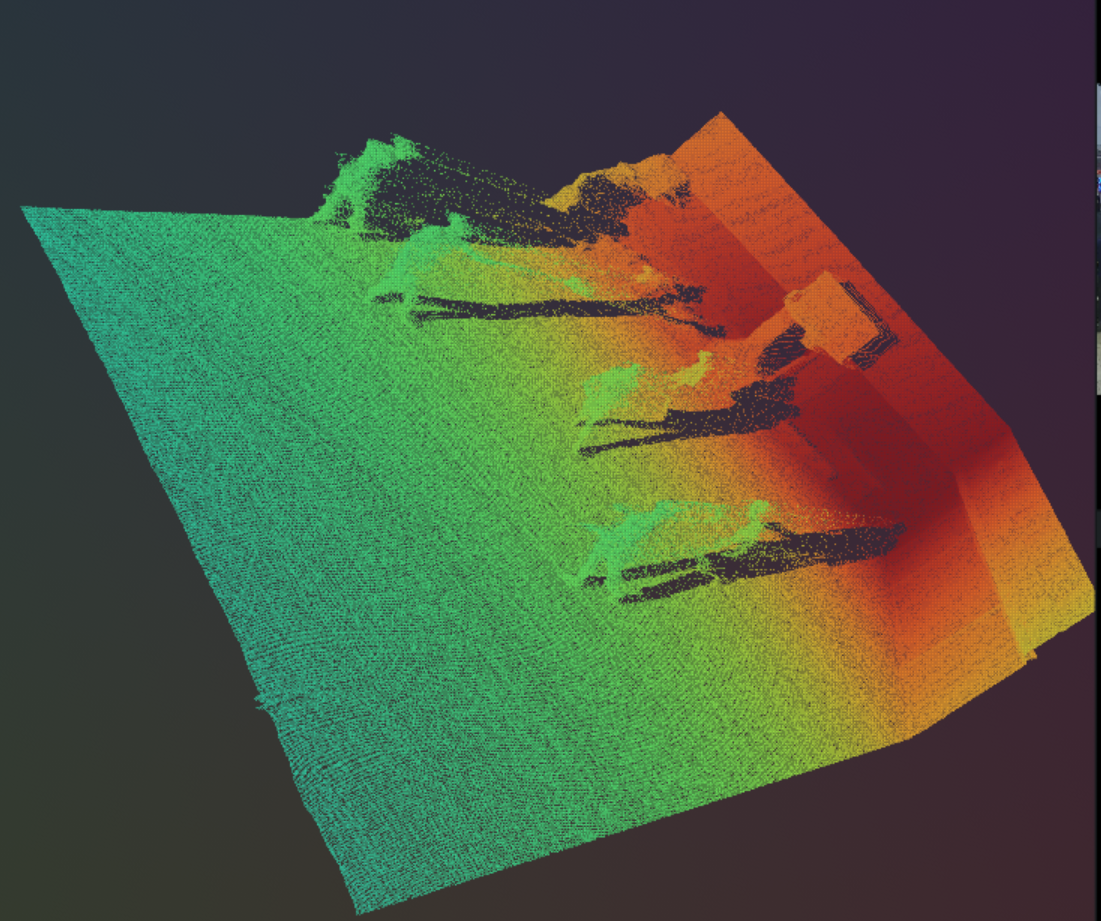
\includegraphics[width=\textwidth]{figures/bigger_view.png}
        \caption{局部放大 (左上区域)}
      \end{figure}
    \end{column}
  \end{columns}
\end{frame}

\begin{frame}{问题分析与下一步}
  \begin{columns}[T]
    \begin{column}{0.5\textwidth}
      \textbf{当前问题}
      \begin{enumerate}
        \item \textbf{多视角未融合}
        \begin{itemize}
          \item 两个视角分别重建
          \item 未形成完整场景
        \end{itemize}
        \item \textbf{Query points 错位}
        \begin{itemize}
          \item 查询点聚集在一起
          \item 位置与场景不匹配
        \end{itemize}
        \item \textbf{可能原因}
        \begin{itemize}
          \item 相机参数设置不正确
          \item 场景归一化范围问题
        \end{itemize}
      \end{enumerate}
    \end{column}
    \begin{column}{0.5\textwidth}
      \textbf{下一步计划}
      \begin{itemize}
        \item 检查相机内外参配置
        \item 调整场景归一化参数
        \item 参考官方配置文件
        \item 尝试不同深度估计方法
      \end{itemize}
      
      \vspace{0.3cm}
      \textbf{VGGT 备选方案}
      \begin{figure}
        \centering
        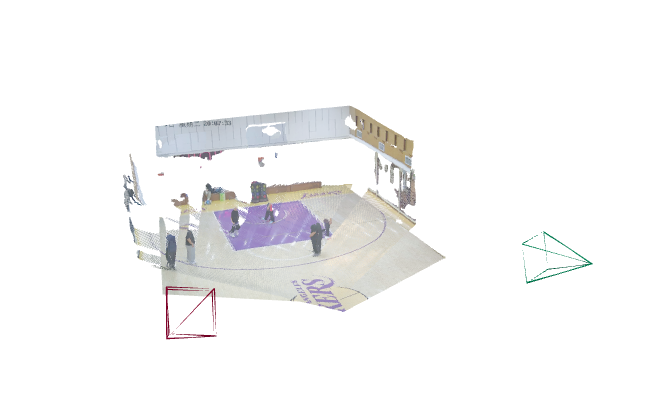
\includegraphics[width=0.8\textwidth]{figures/vggt_demo.png}
        \caption{牛学长 Demo}
      \end{figure}
    \end{column}
  \end{columns}
\end{frame}

\section{TODO}

\begin{frame}{TODO}
  \begin{itemize}
    \item （牛学长建议）先尝试简单方法：ReID模型特征匹配+匈牙利算法解决解决跨视角追踪问题
    \item 调研 MTMCT
    \item 重建效果优化，或尝试使用 VGGT，重建对生成二维战术图有很大帮助
    \item 尝试使用 clip 模型进行 ReID，解决人脸遮挡问题
  \end{itemize}
\end{frame}

\begin{frame}[allowframebreaks]{参考文献}
  \bibliographystyle{thubeamer}
  \bibliography{reference}
\end{frame}

\begin{frame}
  \begin{center}
    {\Huge\calligra Thanks for your attention!}
  \end{center}
\end{frame}

% 结束文档撰写
\end{document}
